\documentclass{article}
 \usepackage{graphicx} 
 \usepackage{amsfonts}
\usepackage{amsmath}
\usepackage{calrsfs}
\usepackage[T1]{fontenc}
\date{}
 \usepackage[colorlinks,urlcolor=blue]{hyperref} 
  \usepackage[left=1.2in,right=1in,top=1in,bottom=.8in]{geometry}
 \date{}
 \title{Project 1 }
\begin{document}
\maketitle

The goal of this work is to find a model from the data of regression data.csv that fit best with the data of yXtest.cvs.

Various attempts have been made.

Those contributing to the final model are explained in the first lines of this file.

By combining Lasso and Random forest regression, I'm trying to beat a Lasso and Ridge baseline to show that there are nonlinear components.

First I tried to use sequentially Lasso then Random Forest. But the results was poor.

By noticing with the Lasso path that the first four characteristics were distinguished, I tried to find the best regularizers which made it possible to best represent these four coefficients without removing too much necessary information.

Then I realized that these parameters were linked so I had to do cross validation by checking them simultaneously.

This is what I did in the estimate reg RERFs.py file. 

While saving the best parameters for lasso and for ridge and for the method combining the two.

That is to say the one which, according to a given lasso regularizator, results in a model which best approximates the penalized data in the sense of lasso and finds a set of regression trees which best approximates what remains after lasso.

It turns out, bad luck that, in my final results, I find the same regularizer for lasso (baseline) and for the lasso used in the combination of the two methods. (0.2364)

But in the most favorable case (0.51 of accuracy of the test set) that I lost, by restarting my cross-validation (with fewer parameters due to lack of computing power).
The two regulators were separate. 



With the parameters found with this cross validation, I compared the models with another cross validation. (compare.py)

This gives the figure given below.

With great joy, we notice that the baseline is beaten.
So there are nonlinear coefficients.

Using the found parameters I train my model in the model.py file that I test in the test.py file.

Thus I find a precision of 0.498 for the model combining the two methods.
I also find 0.443 for lasso only and 0.4322 for Ridge regression.

To find the linear coefficients, it suffices to look at the values ​​of the coefficients of the Lasso models. To find the nonlinear coefficients, it suffices to study which characteristic the forest highlights.




\begin{figure}
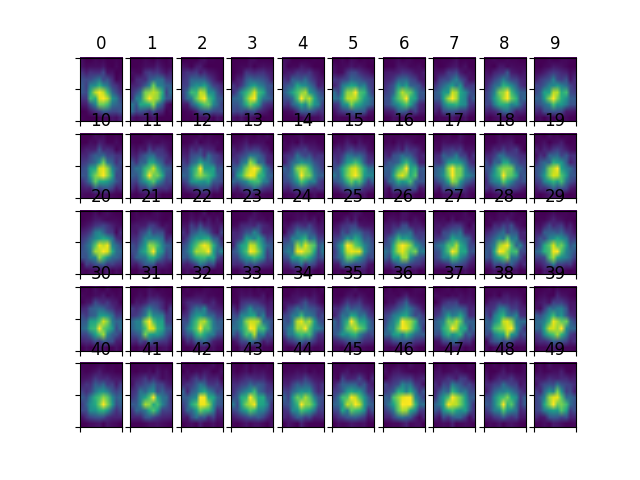
\includegraphics[scale=1]{visu_feature.png}

this figure is a histogram of the features (of the training) with its target.
We note that for the first 4 components there is a preferential direction so there is a great chance that there are linear components.
\end{figure}

\clearpage
\begin{figure}
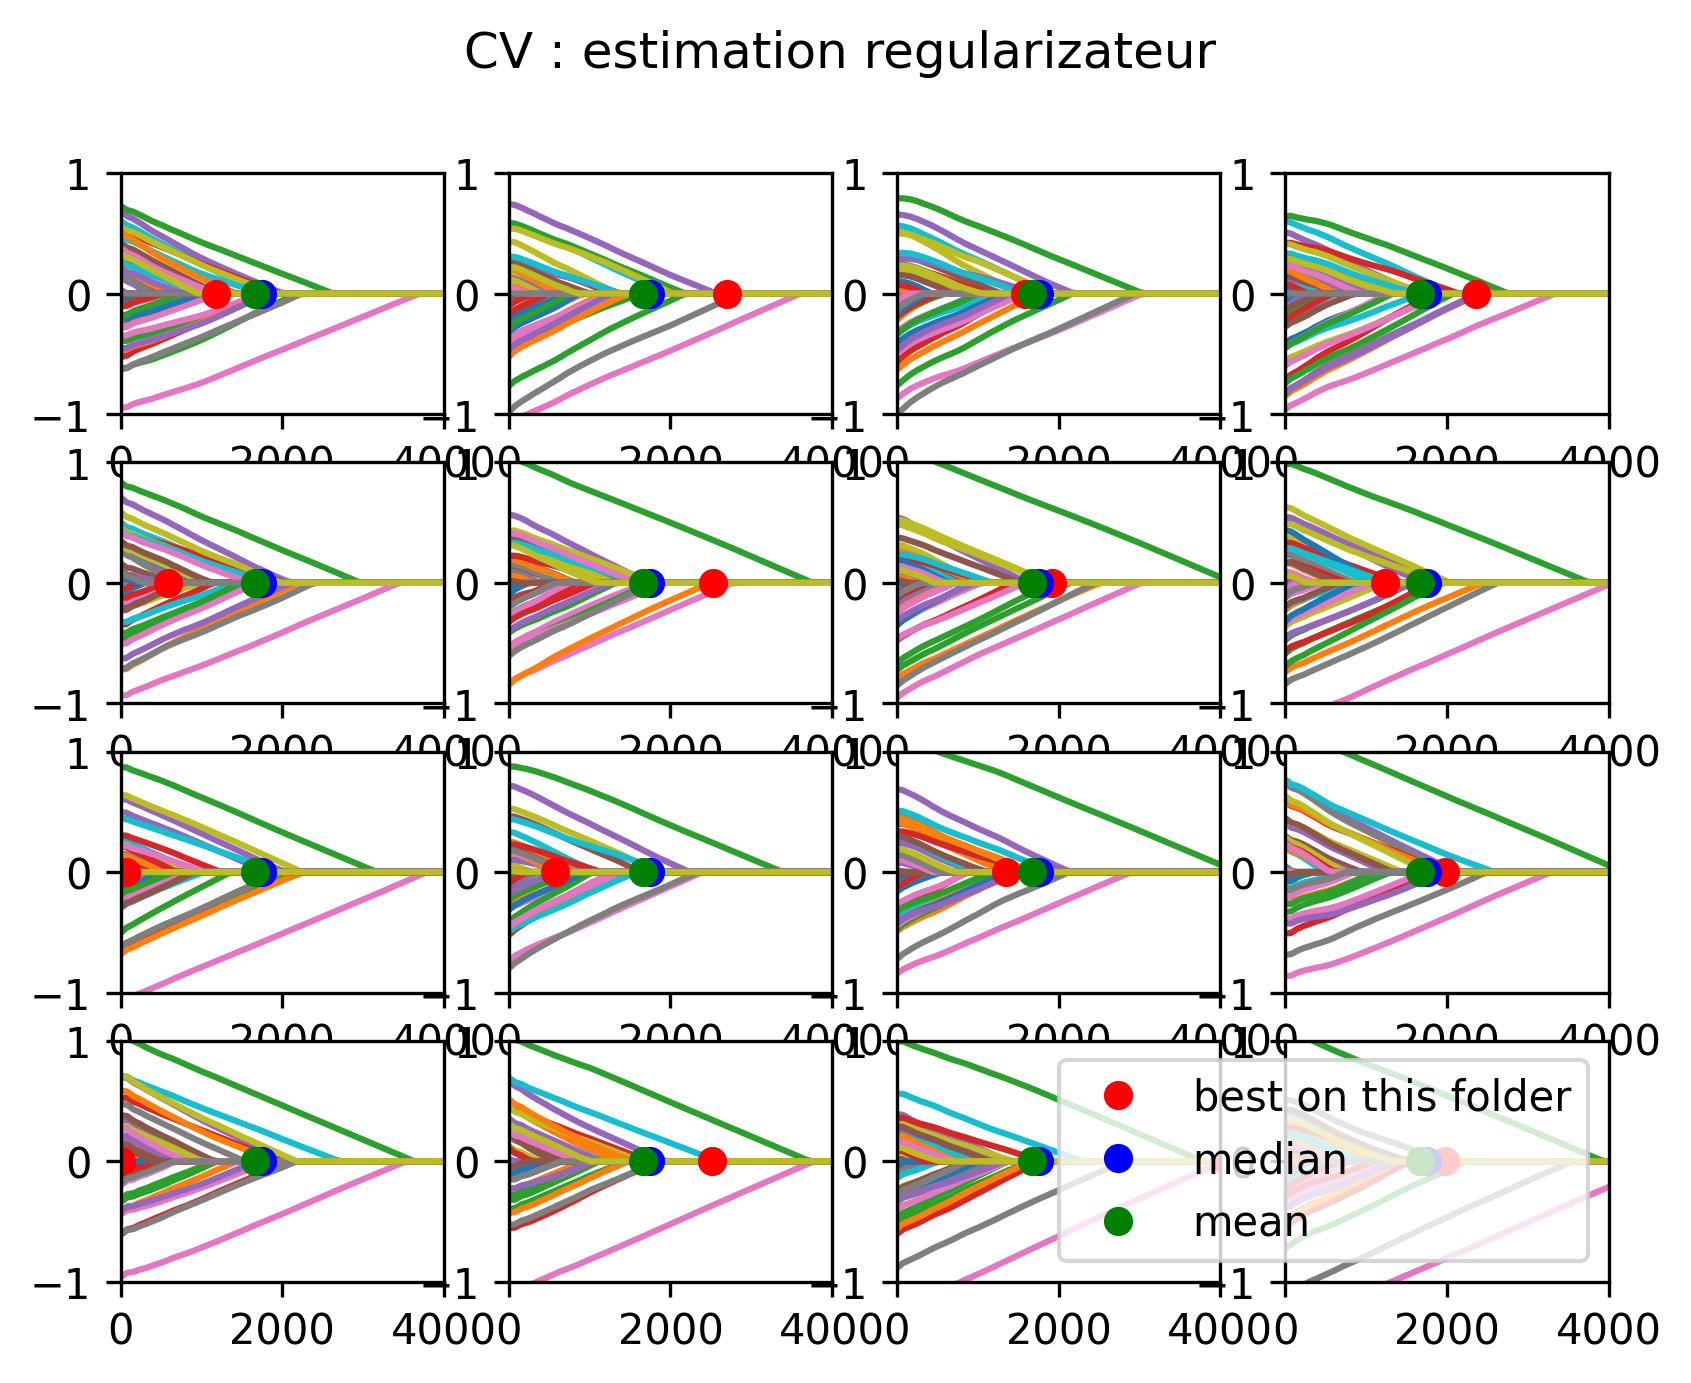
\includegraphics[scale=1]{cv_reg.png}

This figure represents a lasso path during cross-validation.
It allowed me to realize that the first 4 components were surely linear.
\end{figure}
\clearpage

\begin{figure}
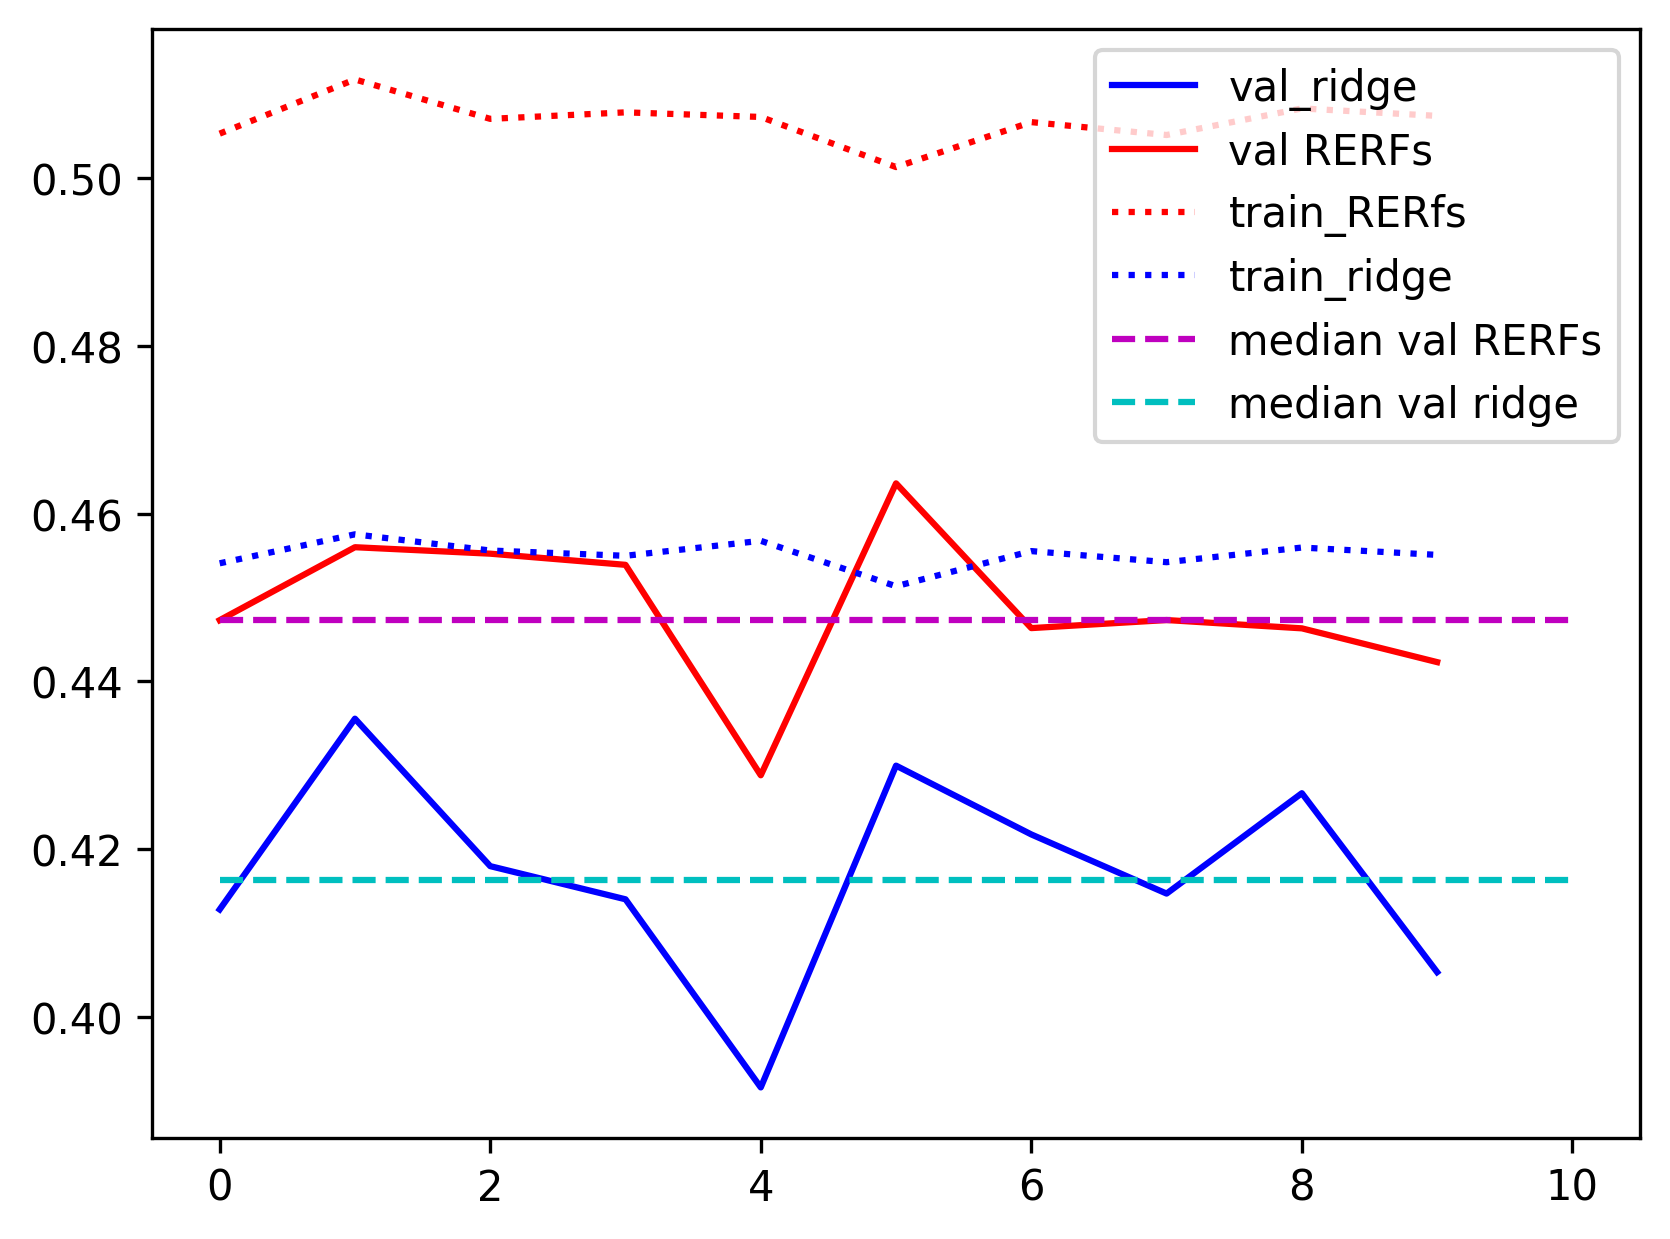
\includegraphics[scale=1]{compare.png}

this figure represents the comparison with the baseline with cross-validations
\end{figure}


\clearpage
\begin{figure}
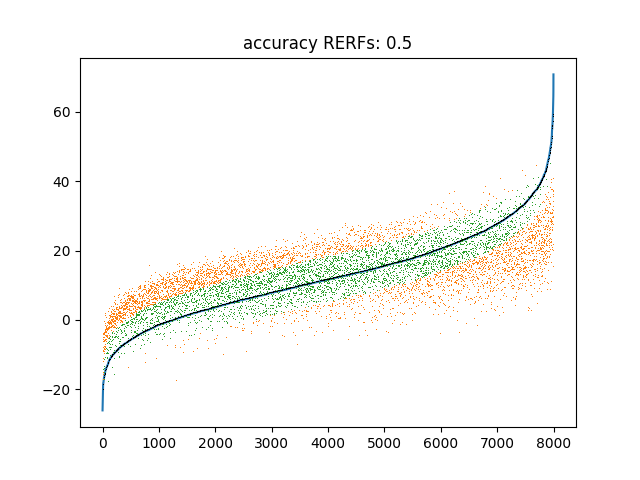
\includegraphics[scale=0.5]{pred_RERFsvs_true.png}
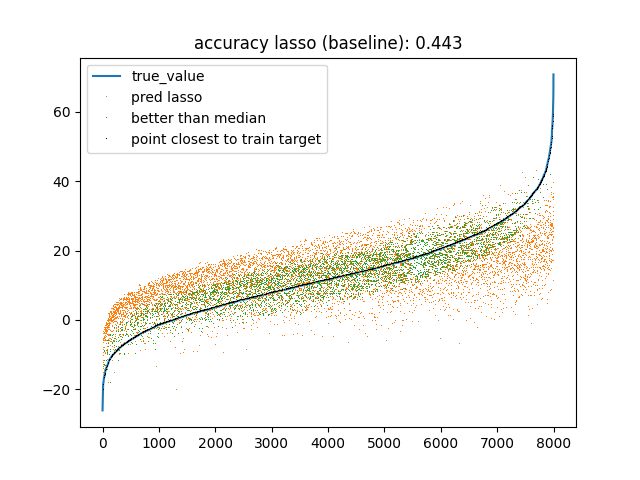
\includegraphics[scale=0.5]{pred_lasso_vs_true.png}
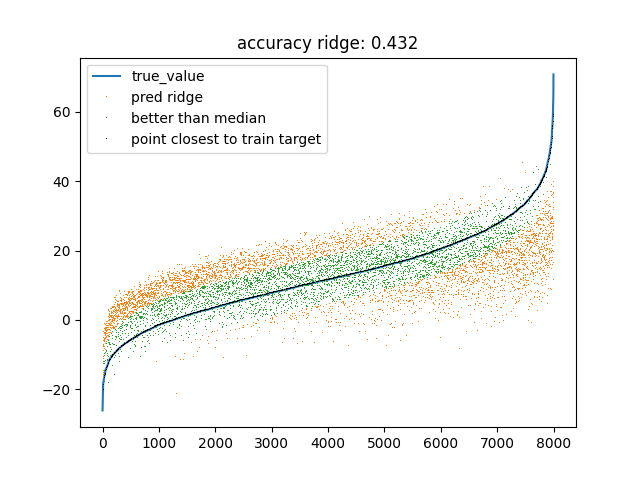
\includegraphics[scale=0.5]{pred_ridge_vs_true.png}

These figures represent the test target ordered and the values ​​of the predictions of the different methods used.

Note: what is in green are the precision values ​​better than the median.

\end{figure}

\newpage


\begin{figure}
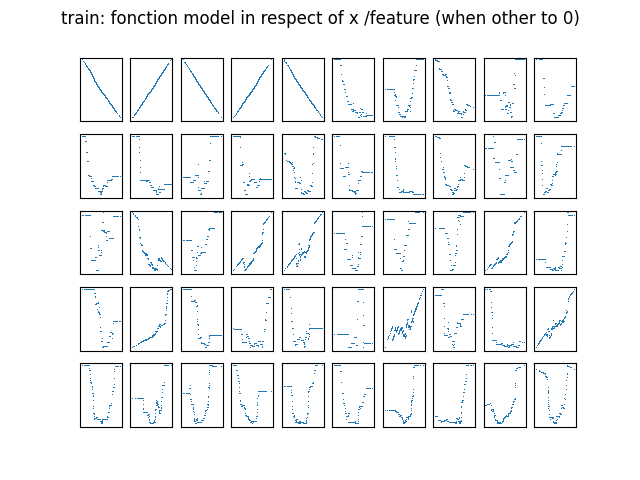
\includegraphics[scale=1]{train_affichage_fonction.png}
\end{figure}

\newpage

\begin{figure}
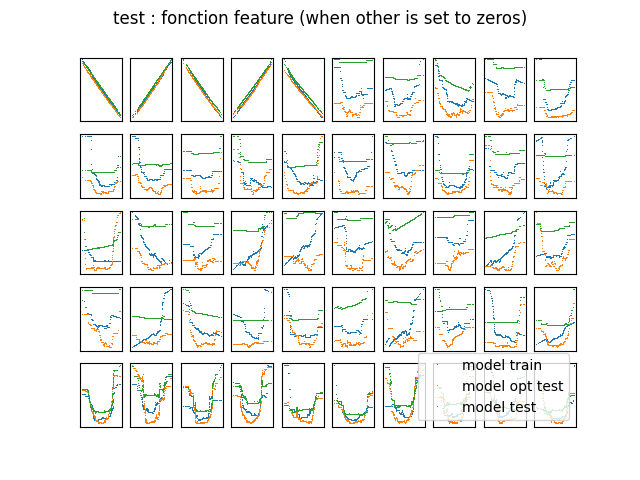
\includegraphics[scale=1]{test_affichage_fonction.png}

Representation of the outputs of the values ​​of the characteristics taken individually.

In addition to best represent the functions, I applied to the test set the model with the parameters found before (model test with 0.61 accuracy)

The other model is a model I built to overfit the data to represent linear and nonlinear coefficients (model opt: accuracy 0.95)

note : 

blue : model train,

orange : opt test model 

vert : model test

\end{figure}

\newpage

\begin{figure}
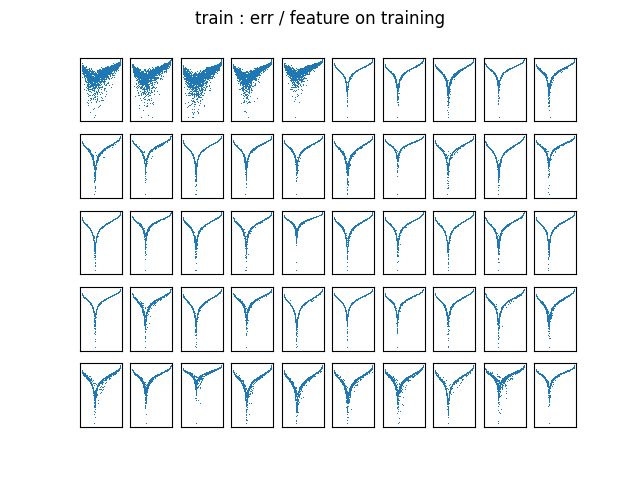
\includegraphics[scale=1]{train_error_par_feature.png}
\end{figure}

\newpage

\newpage

\begin{figure}
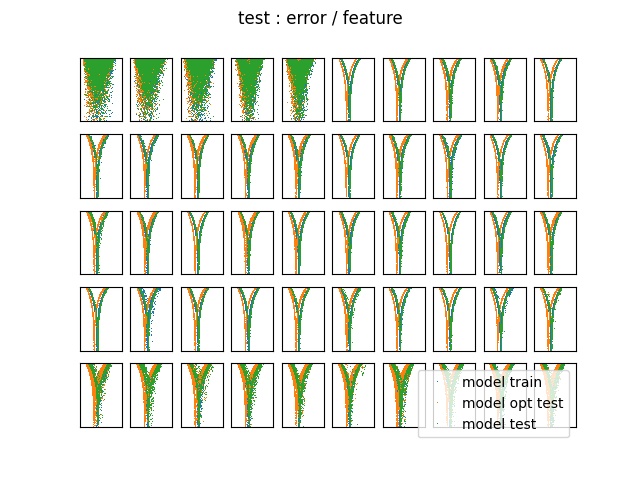
\includegraphics[scale=1]{test_error_par_feature.png}

 We note here that the errors are found on the extremal errors of the targets.


note : 

blue model train

orange : model opt

green : model test
\end{figure}

\newpage


\begin{figure}
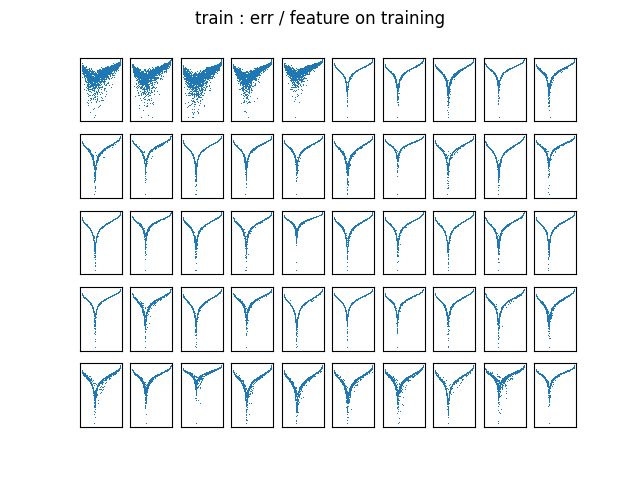
\includegraphics[scale=1]{train_error_par_feature.png}
\end{figure}


\newpage

\begin{figure}
%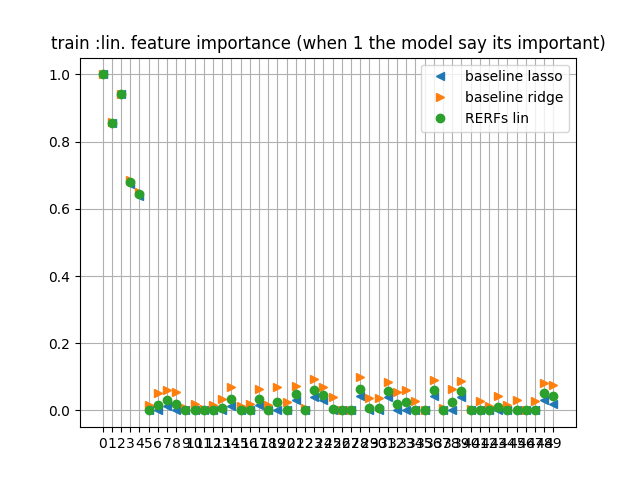
\includegraphics[scale=0.7]{train_linear_feature_importance.png}

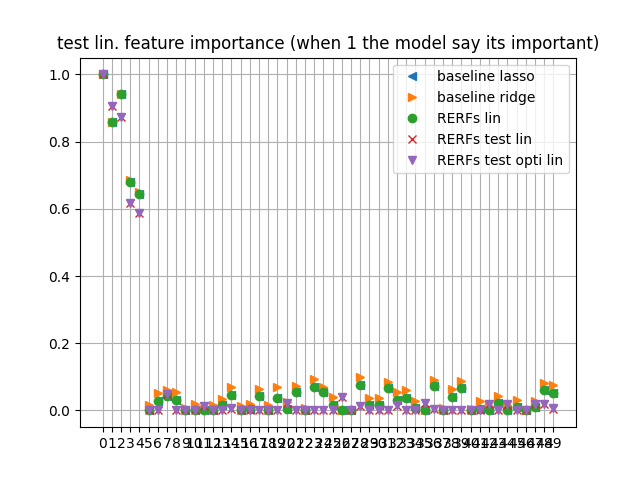
\includegraphics[scale=1]{test_linear_feature_importance.png}

Graphical representation of the role of features in the representation of models.
\end{figure}

\newpage

\begin{figure}
%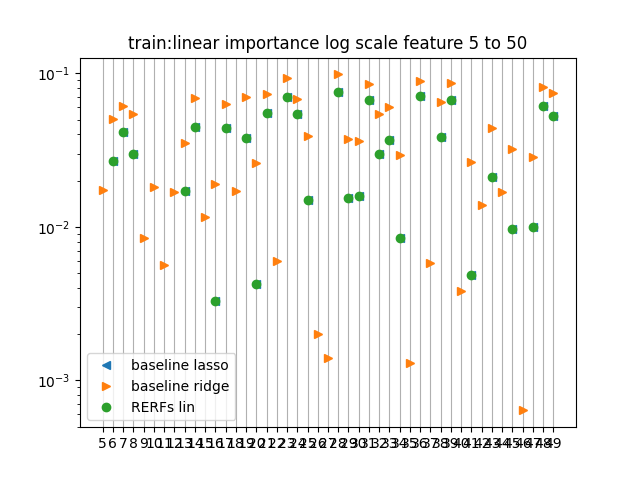
\includegraphics[scale=0.7]{train_linear_feature_importance2.png}

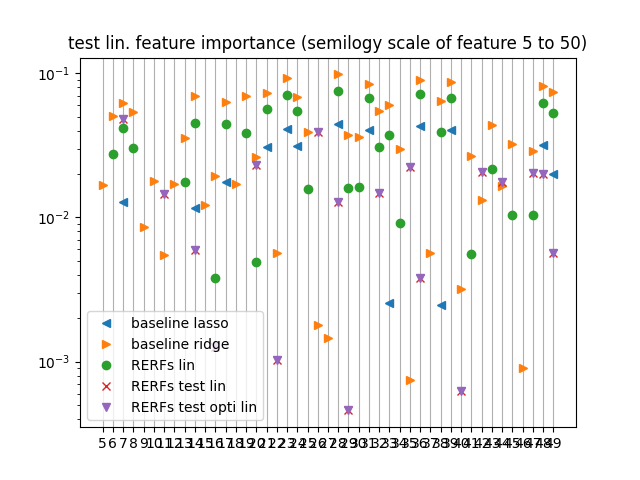
\includegraphics[scale=1]{test_linear_feature_importance2.png}
\end{figure}

\newpage
\begin{figure}
%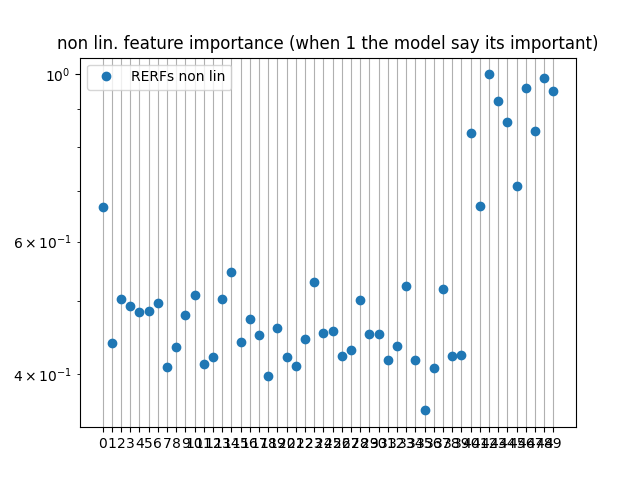
\includegraphics[scale=0.7]{train_non_linear_feature_importance.png}

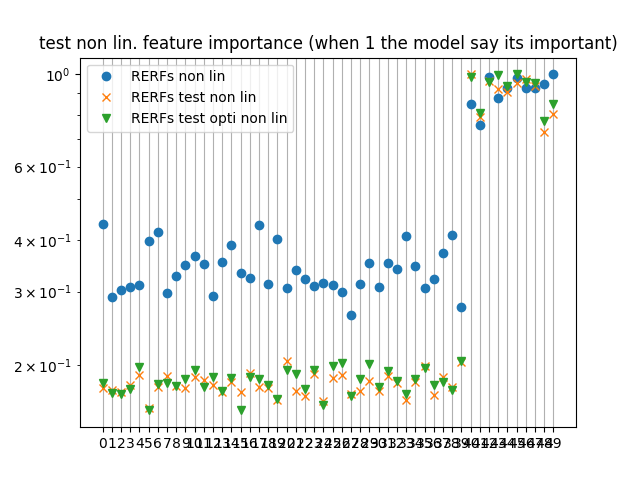
\includegraphics[scale=1]{test_non_linear_feature_importance.png}
\end{figure}


\end{document}